% Options for packages loaded elsewhere
\PassOptionsToPackage{unicode}{hyperref}
\PassOptionsToPackage{hyphens}{url}
%
\documentclass[
]{article}
\usepackage{amsmath,amssymb}
\usepackage{lmodern}
\usepackage{iftex}
\ifPDFTeX
  \usepackage[T1]{fontenc}
  \usepackage[utf8]{inputenc}
  \usepackage{textcomp} % provide euro and other symbols
\else % if luatex or xetex
  \usepackage{unicode-math}
  \defaultfontfeatures{Scale=MatchLowercase}
  \defaultfontfeatures[\rmfamily]{Ligatures=TeX,Scale=1}
\fi
% Use upquote if available, for straight quotes in verbatim environments
\IfFileExists{upquote.sty}{\usepackage{upquote}}{}
\IfFileExists{microtype.sty}{% use microtype if available
  \usepackage[]{microtype}
  \UseMicrotypeSet[protrusion]{basicmath} % disable protrusion for tt fonts
}{}
\makeatletter
\@ifundefined{KOMAClassName}{% if non-KOMA class
  \IfFileExists{parskip.sty}{%
    \usepackage{parskip}
  }{% else
    \setlength{\parindent}{0pt}
    \setlength{\parskip}{6pt plus 2pt minus 1pt}}
}{% if KOMA class
  \KOMAoptions{parskip=half}}
\makeatother
\usepackage{xcolor}
\usepackage[margin=1in]{geometry}
\usepackage{graphicx}
\makeatletter
\def\maxwidth{\ifdim\Gin@nat@width>\linewidth\linewidth\else\Gin@nat@width\fi}
\def\maxheight{\ifdim\Gin@nat@height>\textheight\textheight\else\Gin@nat@height\fi}
\makeatother
% Scale images if necessary, so that they will not overflow the page
% margins by default, and it is still possible to overwrite the defaults
% using explicit options in \includegraphics[width, height, ...]{}
\setkeys{Gin}{width=\maxwidth,height=\maxheight,keepaspectratio}
% Set default figure placement to htbp
\makeatletter
\def\fps@figure{htbp}
\makeatother
\setlength{\emergencystretch}{3em} % prevent overfull lines
\providecommand{\tightlist}{%
  \setlength{\itemsep}{0pt}\setlength{\parskip}{0pt}}
\setcounter{secnumdepth}{5}
\newlength{\cslhangindent}
\setlength{\cslhangindent}{1.5em}
\newlength{\csllabelwidth}
\setlength{\csllabelwidth}{3em}
\newlength{\cslentryspacingunit} % times entry-spacing
\setlength{\cslentryspacingunit}{\parskip}
\newenvironment{CSLReferences}[2] % #1 hanging-ident, #2 entry spacing
 {% don't indent paragraphs
  \setlength{\parindent}{0pt}
  % turn on hanging indent if param 1 is 1
  \ifodd #1
  \let\oldpar\par
  \def\par{\hangindent=\cslhangindent\oldpar}
  \fi
  % set entry spacing
  \setlength{\parskip}{#2\cslentryspacingunit}
 }%
 {}
\usepackage{calc}
\newcommand{\CSLBlock}[1]{#1\hfill\break}
\newcommand{\CSLLeftMargin}[1]{\parbox[t]{\csllabelwidth}{#1}}
\newcommand{\CSLRightInline}[1]{\parbox[t]{\linewidth - \csllabelwidth}{#1}\break}
\newcommand{\CSLIndent}[1]{\hspace{\cslhangindent}#1}
\ifLuaTeX
  \usepackage{selnolig}  % disable illegal ligatures
\fi
\IfFileExists{bookmark.sty}{\usepackage{bookmark}}{\usepackage{hyperref}}
\IfFileExists{xurl.sty}{\usepackage{xurl}}{} % add URL line breaks if available
\urlstyle{same} % disable monospaced font for URLs
\hypersetup{
  pdftitle={Evaluating Clustering Techniques on Non-elliptical Data},
  pdfauthor={Safiya Sirota, Yijin Wang, Bin Yang},
  hidelinks,
  pdfcreator={LaTeX via pandoc}}

\title{Evaluating Clustering Techniques on Non-elliptical Data}
\author{Safiya Sirota, Yijin Wang, Bin Yang}
\date{}

\begin{document}
\maketitle

{
\setcounter{tocdepth}{2}
\tableofcontents
}
\hypertarget{background-and-objective}{%
\section{Background and Objective}\label{background-and-objective}}

Latent Class Analysis and K-means are two successful clustering
algorithms that partition the given data into distinct subgroups where
observations in each group are very similar. They are popular choice of
method in solving healthcare research problems such as identifying
clusters on microscopic images (Amin et al. 2015), categorizing suicides
by risk factors (Logan, Hall, and Karch 2011), and grouping elderly
patients with their access to health care (Thorpe et al. 2011). One
important assumption that both of these algorithms require is the
normality of the given data.

In our project, we focus on the unsupervised learning scenario and we
investigate how well these two algorithms perform when the normality
assumption is violated. We designed 4 simulation settings as violation
of the normality assumption: 1) skewed data, 2) data with heavy tail, 3)
data with outliers, 4) multimodal data. In the end, we compare their
performance with Rand Index in each settings with varying sample sizes.

\hypertarget{statistical-method}{%
\section{Statistical Method}\label{statistical-method}}

\hypertarget{k-means}{%
\subsection{K Means}\label{k-means}}

\hypertarget{latent-class-analysis}{%
\subsection{Latent Class Analysis}\label{latent-class-analysis}}

\hypertarget{performance-metric}{%
\section{Performance Metric}\label{performance-metric}}

\hypertarget{simulations-settings-and-results}{%
\section{Simulations Settings and
Results}\label{simulations-settings-and-results}}

In simulations, we consider bivariate data with 2 true clusters. We
generated data from different non-elliptical distributions in each
setting.

For each simulation setting, we create 100 runs using randomly generated
data sets in size of 500, 1000, 5000 and evaluate the Rand index for
each method.

\hypertarget{skewed-data---data-generation}{%
\subsection{Skewed Data - Data
Generation}\label{skewed-data---data-generation}}

In this setting, we want to test the performance of K-means and LCA when
all features follow a skewed distribution. We assume the features
\(X_1, X_2\) are independent.

All data in the first feature \(X_{11}, X_{12},..X_{1N}\) are random
draws from a mixture model of Weibull distributions with density
\(0.5f_1(x|1,5) + 0.5f_2(x|12,14)\) where \(f_1 \sim Weibull(1,5)\) and
\(f_2 \sim Weibull (12,14)\).

Similarly, all data in the second feature \(X_{21}, X_{22},..X_{2N}\)
are random draws from another mixture model of Weilbull distributions
with density \(0.5f_3(x|1,3) + 0.5f_4(x|1,4)\) where
\(f_3 \sim Weibull(1,3)\) and \(f_4 \sim Weibull (1,4)\).

We generate 2 equal-sized clusters with total size being 500, 1000 and
5000. An example of a sample with size 5000 is shown below.

\begin{figure}
\centering
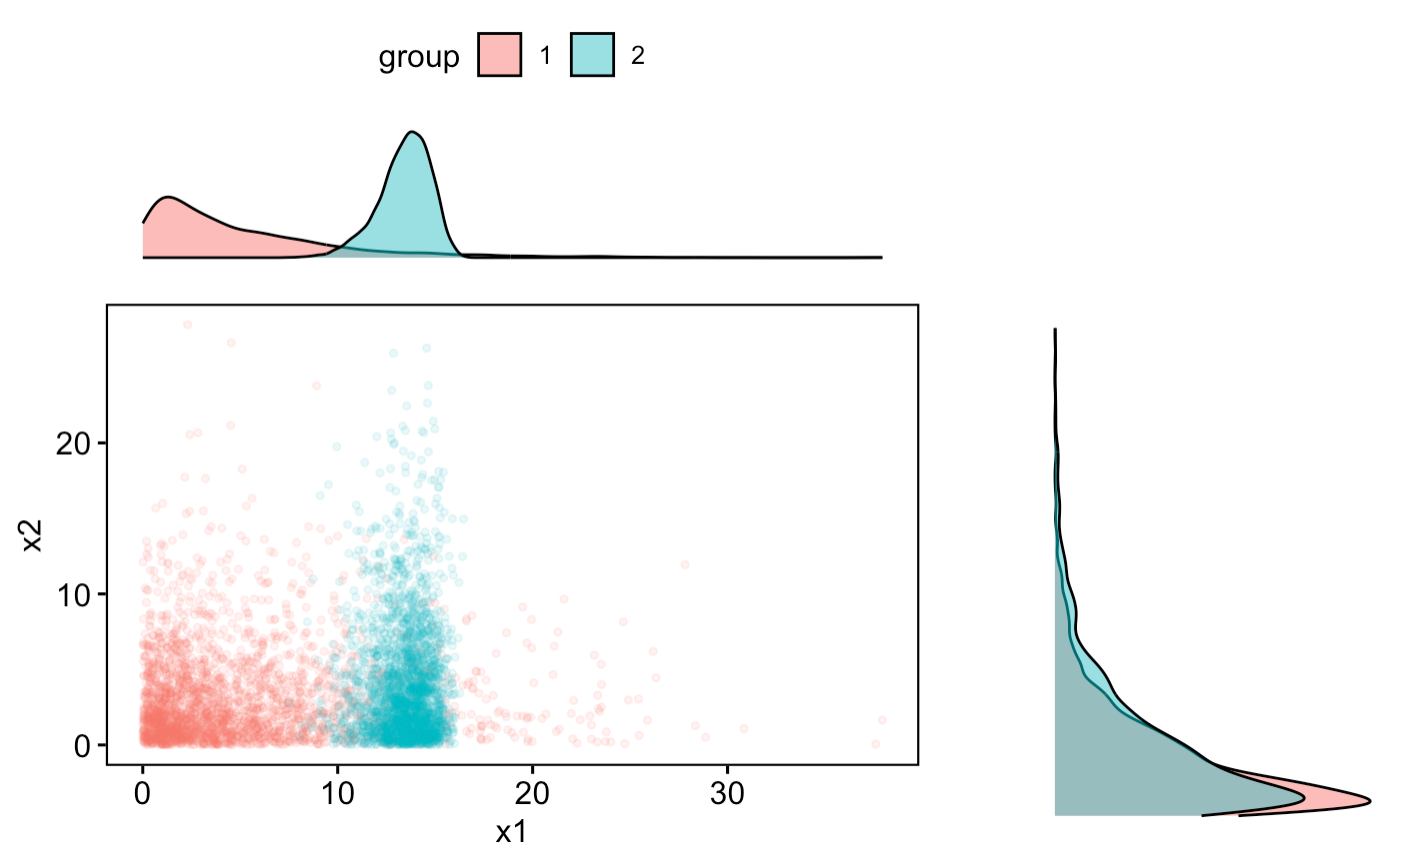
\includegraphics[width=4.16667in,height=\textheight]{report_image/skewed_sample.png}
\caption{Skewed Data Sample}
\end{figure}

\hypertarget{skewed-data---results}{%
\subsection{Skewed Data - Results}\label{skewed-data---results}}

We are interested in how well K-means and LCA perform when the input
data already has two true clusters. We calculate Rand Index for sample
data in each simulation run and conclude that after 100 simulations,
K-means performs better than LCA across all sample sizes. As sample size
increases, the variance of Rand Index decreases.

\begin{figure}
\centering
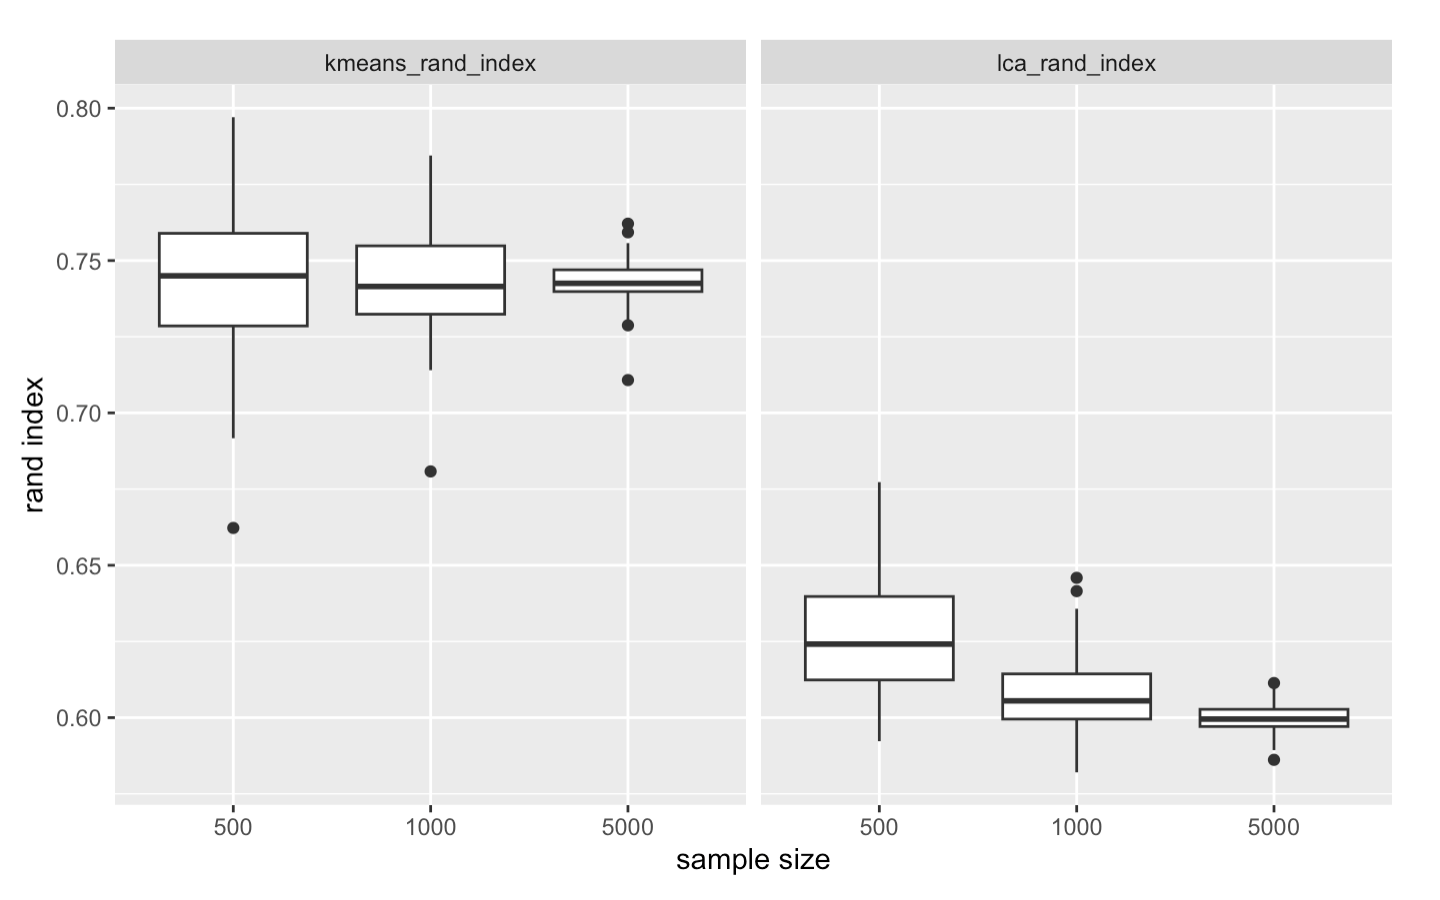
\includegraphics[width=4.16667in,height=\textheight]{report_image/skewed_data_rand_index_results.png}
\caption{Skewed Data Comparison - Rand Index}
\end{figure}

To investigate some potential reasons behind this, we compare the
optimal number of cluster number for each method in all simulations.
Choosing the optimal cluster number is the first step for both methods.
This number is crucial to our comparison because we predetermined the
number of true clusters to be 2 and Rand Index uses the number of
agreements in its calculation. Therefore, having a cluster number that
is larger than 2 could hurt the performance.

In this figure, we compare the optimal number of clusters. Overall,
K-means choose its optimal number of cluster around 3 which is much
lower than that of LCA across all sample sizes. As sample size
increases, the optimal number of cluster increases for LCA as well.

\begin{figure}
\centering
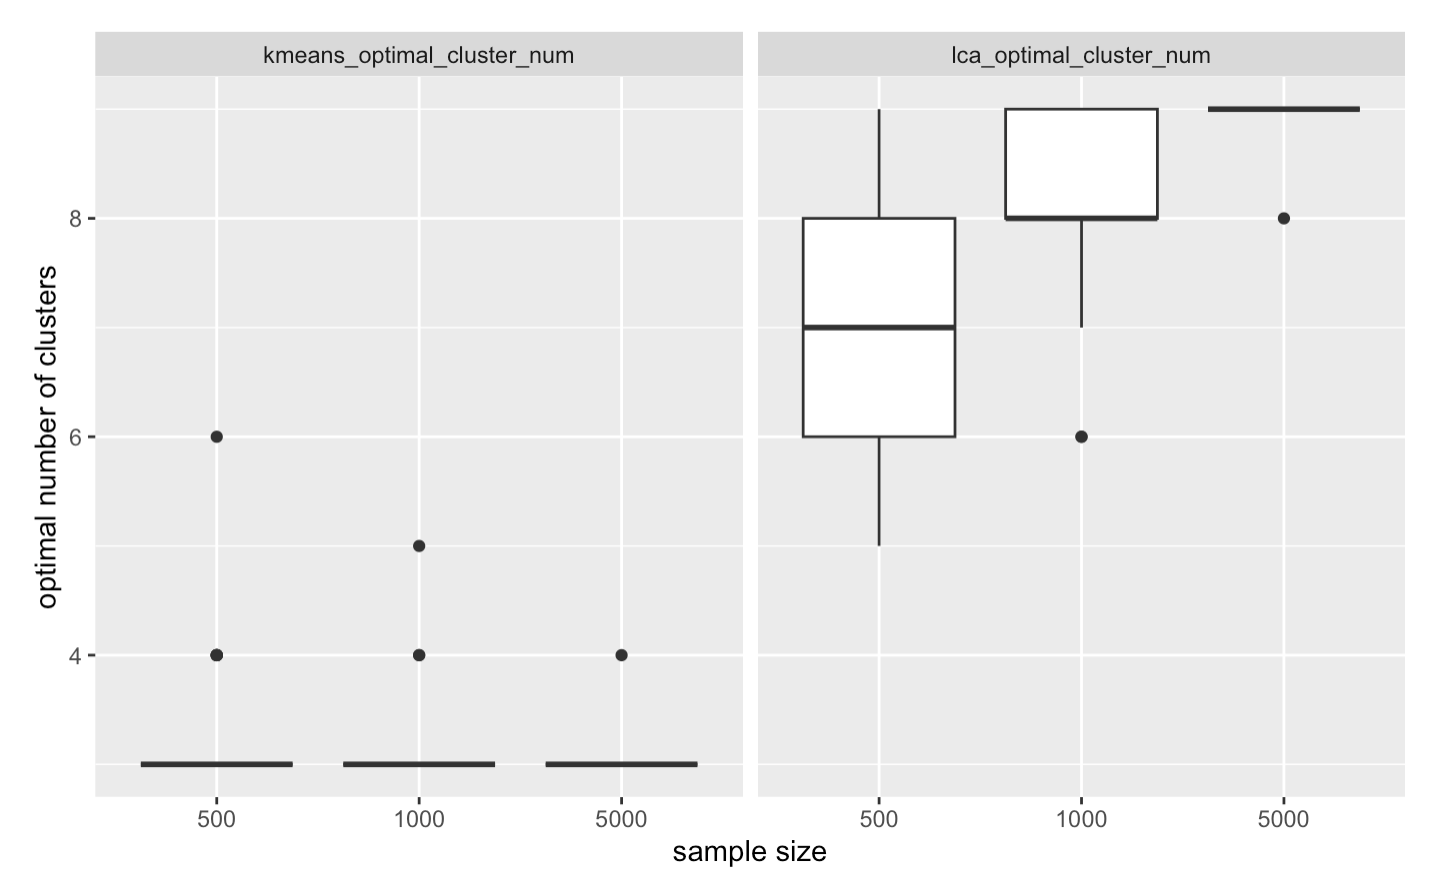
\includegraphics[width=4.16667in,height=\textheight]{report_image/skewed_data_num_clusters_results.png}
\caption{Skewed Data Comparison - Optimal Number of Clusters}
\end{figure}

\hypertarget{conclusion-and-discussion}{%
\section{Conclusion and Discussion}\label{conclusion-and-discussion}}

\hypertarget{references}{%
\section{References}\label{references}}

\hypertarget{refs}{}
\begin{CSLReferences}{1}{0}
\leavevmode\vadjust pre{\hypertarget{ref-amin_recognition_2015}{}}%
Amin, Morteza Moradi, Saeed Kermani, Ardeshir Talebi, and Mostafa
Ghelich Oghli. 2015. {``Recognition of {Acute} {Lymphoblastic}
{Leukemia} {Cells} in {Microscopic} {Images} {Using} {K}-{Means}
{Clustering} and {Support} {Vector} {Machine} {Classifier}.''}
\emph{Journal of Medical Signals and Sensors} 5 (1): 49--58.
\url{https://www.ncbi.nlm.nih.gov/pmc/articles/PMC4335145/}.

\leavevmode\vadjust pre{\hypertarget{ref-logan_suicide_2011}{}}%
Logan, Joseph, Jeffrey Hall, and Debra Karch. 2011. {``Suicide
{Categories} by {Patterns} of {Known} {Risk} {Factors}: {A} {Latent}
{Class} {Analysis}.''} \emph{Archives of General Psychiatry} 68 (9):
935--41. \url{https://doi.org/10.1001/archgenpsychiatry.2011.85}.

\leavevmode\vadjust pre{\hypertarget{ref-thorpe_patterns_2011}{}}%
Thorpe, Joshua M., Carolyn T. Thorpe, Korey A. Kennelty, and Nancy
Pandhi. 2011. {``Patterns of Perceived Barriers to Medical Care in Older
Adults: A Latent Class Analysis.''} \emph{BMC Health Services Research}
11 (1): 181. \url{https://doi.org/10.1186/1472-6963-11-181}.

\end{CSLReferences}

\end{document}
